
\chapter{Design \& Methodology\label{ch:usage}}
Debloating has been applied to different parts of the software stack ranging from operating systems to containers and even executable binaries. Likewise, we also expect the web applications to benefit from this method of attack surface reduction.
To quantify the extend to which various web applications are affected by debloating is the main research question of this study. The general architecture of web applications and their attack vectors are different than binaries.
Based on this observation, debloating mechanisms that remove dead code and make exploitation harder by reducing the number of available gadgets only provide marginal benefit. By removing the actual vulnerabilities, we can cover a wider range of attacks.

Furtheremore, web applications are inherently more dynamic than compiled binaries. Decisions are made on the fly and its typical to dynamically load code at runtime. This makes static analysis even more complicated and less accurate. As a result, we rely on dynamic analysis and usage profiling to detect bloat. In the remainder of this section, we take a look at code reuse and external dependencies as the main source of bloat for web applications, and then describe the design and implementation details of our debloating pipeline.
\section{Background}
We briefly describe the effect of package managers on software
bloat and provide a motivating example for debloating web applications.


\subsection{Package managers and software bloat}
To ease the development of software, developers reuse third-party libraries,
external packages, and frameworks for their applications. This approach
enables developers to focus on their applications while relying on
proven and tested components. Statistics from popular package managers show
that reliance on external packages is a widely adopted practice across
many different languages. NPM, the registry hosting NodeJS packages,
reports more than 10 billion package downloads a
month~\cite{nodeDownloads}. Similarly, PyPI, the package manager for Python,
reports more than a billion a month~\cite{pypiDownloads}, while Packagist, the main repository for
Composer package manager for PHP, reports the download of 500 million
packages each month~\cite{packagistDownloads}.

At the same time, it is doubtful that \emph{all} the code and features
obtained through these packages and frameworks are actually used by
the applications that rely on them. For the most part, when developers rely on
external dependencies, they include entire packages with no effective way of
disabling and/or removing the parts of these packages and frameworks that
their applications do not require.

\subsection{Motivating web-application debloating}

In this study, we look at the bloat of web applications and quantify how
debloating can provide concrete security benefits. Even
though debloating has been successfully applied in other contexts, we argue
that the
idiosyncrasies of the web platform (e.g. the ambient authority of cookies and
the client/server model which is standard for the web but atypical
for operating systems and compiled software) require a dedicated analysis
of the applicability of debloating for web applications.

%As detailed in Section~\ref{sec:related}, several works have been
%published in the debloating domain but none of them looked specifically
%at web applications, nor did they tackle the subject from a security
%perspective. Indeed, web applications are vulnerable to different classes
%of attacks like code execution, denial of service or authentication bypass.
%Understanding the impact of debloating requires its own in-depth analysis
%that cannot be derived from other types of applications. Since we focus on
%the business logic of web applications, we decided upon PHP as the language
%used for this study. It is one of the most widely used server-side language
%in the world~\cite{phpAdoption} and very popular websites like Facebook,
%Yahoo or Wikipedia have a large part of their codebase written in this
%language. A package manager called Composer handles external dependencies
%in PHP~\cite{composer} and it relies on packages hosted on the Packagist
%website~\cite{packagist}.



To understand how the bloat of a web application can lead to a critical
vulnerability, we use a recent vulnerability of the Symfony web
framework (CVE-2018-14773~\cite{symfonyVulnerability}) as a motivating
example. Specifically, the Symfony web framework supported a legacy IIS
header that could be abused to have Symfony return a different URL than the
one in the request header, allowing the bypassing of web application firewalls
and server-side access-control mechanisms. If this type of header
was never used by the server, debloating the application would have removed
support for it, which ultimately would have prevented anyone from exploiting
the vulnerability. Drupal, a popular PHP Content Management System (CMS), was also affected by
the same vulnerability since it uses libraries from the Symfony framework
to handle parts of its internal logic~\cite{drupalVulenrability}. Even
if Drupal developers were not responsible for the code that leads to the
vulnerability, their application could still be exploited since Symfony
was an external dependency. Even more interestingly, an analysis of the
official Symfony patch on GitHub~\cite{symfonyPatch}
reveals that the vulnerable lines were derived from yet another framework
called Zend~\cite{zendVulnerability}. This shows that the structure of web
applications can be very complex with code reuse originating from many
different sources. Even if developers take all possible precautions to
minimize vulnerabilities in their own code, flaws from external dependencies
can cascade and lead to a critical entry point for an attacker.

Overall, there are clear benefits that debloating could have on web
applications. Assuming that we are able to pinpoint all the code that is required
by the users of a given software deployment, all other code (including the
code containing vulnerabilities) can be removed from that deployment.

\section{Setup}
In this section, we describe the process of gathering information regarding
known vulnerabilities (in the form of CVEs) for web applications, designing
and executing tests against web applications of interest, and identifying
the server-side code that was executed as a result of client-side actions.


\begin{figure}[t]
  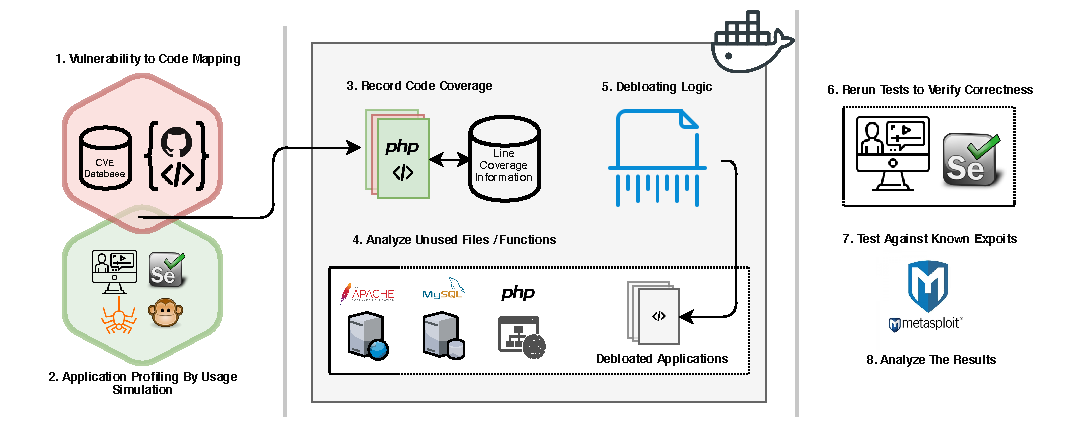
\includegraphics[width=\linewidth]{figures/DebloatingPipeline.pdf}
  \caption{Overview of the architecture of our pipeline for debloating web applications and assessing the effects of different debloating strategies.}
  \label{fig:debloatingpipeline}
\end{figure}

\subsection{Overview}
The setup for our framework is depicted in
Figure~\ref{fig:debloatingpipeline}. To debloat target applications, we first
collect information about the vulnerabilities of the applications that we
analyze in our study. This information includes the files, functions, and
line numbers where each
vulnerability resides (Step 1, Section~\ref{sec:vulntosourcemapping}). Then,
we simulate usage of the application through a combination of different
techniques (Step 2, Section~\ref{subsec:profiling}). Using a PHP profiler
tool (\texttt{XDebug}), we record the lines, functions, and files, that are
triggered during the simulation (Step 3, Section~\ref{subsec:coverage}).

In the middle part of our pipeline, the debloating engine takes both the
target applications and coverage information to perform debloating at
different levels of granularity, and rewrite parts of the application to
remove unused pieces of code based on the debloating strategy being evaluated
(Steps 4 and 5, Section~\ref{sec:debloating}). Our framework also provides
a complete reporting panel to assist human analysts in understanding which
vulnerabilities can be removed by the present debloating strategies.

Last, we verify the correctness of our debloating process by running
a set of tests against the debloated web applications, and verifying that
no removed piece of code is triggered (Step 5). To this end, we
utilize assertions in place of the removed code blocks. An absence of error
messages from these assertions means that all tests were successfully
completed without triggering any missing server-side code. As an final step of
verification, we also test the debloated applications against a series of
exploits and verify that exploits which
abuse any of the vulnerabilities that were removed as part of the debloating
process, do not succeed (Step 6, Section~\ref{section:metasploit}).

To ease integration and facilitate the analysis of new web applications, we
adopted a modular architecture that relies on three Docker containers. The
\textit{Application} container hosts our web applications.  The profiler
enabled on its web server is responsible for collecting code coverage
information. The \textit{Database} container runs a MySQL server that
stores the code coverage information along with the databases of the tested
applications. Lastly, the \textit{Debloating} container which includes our
debloating logic, analyzes the coverage information and generates debloated
versions of applications. It also provides a reporting panel that indicates
which vulnerabilities are removed in each application after debloating. To add
a new vulnerability, a user simply has to provide the details of the vulnerable
file(s) and line(s).


\subsection{Analyzed web applications}
\label{subsec:webapps}

To understand how the process of debloating increases the security of web
applications, we decided against using toy-like web applications. Instead,
we focused on established open-source applications with millions of users,
and the presence of a sufficient number of known historical vulnerabilities
(in the form of CVEs) to allow us to generalize from them. To this end, we
selected {phpMyAdmin}~\cite{phpmyadmin},
{MediaWiki}~\cite{mediawiki}, {Magento}~\cite{magento}, and WordPress~\cite{wordpress},
which are representative samples of four different types of
web applications namely web-administration tools, wikis, online
shops, and blogging software. Table~\ref{table:analyzed_webapps} shows the versions of these web
applications that we utilized, in order to map CVEs to the location of the
vulnerability in the source code of each application.


\begin{table}[]
\centering
\caption{Analyzed open-source web applications.}
\scalebox{0.87}{
\begin{tabular}{|l|l|c|}
\hline
\textbf{Web Application} & \textbf{Version}                            & \begin{tabular}[c]{@{}l@{}}\textbf{Known CVEs}\\\hspace{1em}($\geq$2013)\end{tabular} \\ \hline
Magento                  & 1.9.0, 2.0.5                                 & 10                                                                     \\ \hline
MediaWiki                & 1.19.1, 1.21.1, 1.24.0, 1.28.0 & 111                                                                    \\ \hline
phpMyAdmin               & 4.0.0, 4.4.0, 4.6.0, 4.7.0     & 130                                                                    \\ \hline
WordPress                & 3.9.0, 4.0, 4.2.3, 4.6, 4.7, 4.7.1  & 131                                                                    \\ \hline
\end{tabular}
}
\label{table:analyzed_webapps}
\end{table}

\subsection{Vulnerability to source-code mapping}
\label{sec:vulntosourcemapping}
To determine whether debloating web applications can actually remove
vulnerabilities, we performed a mapping of known CVEs to the vulnerable lines,
functions, and files, that they exploit in each application. This way, by
looking at an application after debloating, we can determine if the files,
functions, or lines responsible for the vulnerability, are still present or
were removed during the debloating process.


Even though there exist multiple databases listing the current and
historical CVEs of popular software (including the web applications in
question)~\cite{cvedetails,nistgov}, locating the actual source code
containing the vulnerability described in a CVE, is a non-trivial process
which requires careful investigation. In some cases, the right patch can be
discovered because of a direct reference to a CVE in a commit message, or in
a bug report on official public repositories of web applications. For others,
the fix is included within numerous commits that have to be carefully analyzed
to locate the appropriate lines of code. Since a vulnerability can span over
multiple lines, functions, and even multiple files, we record all affected
locations in a database so that this information can be later correlated
with each evaluated application.


Given the time-consuming nature of mapping CVEs to existing code, for
this study, we limited ourselves to, at most, 20 CVEs per application
of interest.
The complete list of CVEs we mapped for this study can be found in
Table~\ref{table:listofallcves} in the Appendix.
To select these CVEs, we ordered existing vulnerabilities by
their CVSS score (thereby selecting the ones that are the most critical)
and we did not consider vulnerabilities that were reported before 2013. This
focus on fairly recent vulnerabilities (i.e. in the last five years) makes
our results more generalizable to the current state of web applications,
as opposed to quantifying vulnerabilities in source-code which has since
dramatically evolved. Note that, because not all versions of a web application
are vulnerable to all evaluated CVEs, we had to map vulnerabilities
across a number of different versions, as shown in
Table~\ref{table:analyzed_webapps}.



\subsection{Application usage profiling}
\label{subsec:profiling}

Modern web applications provide an incredibly wide range of features and
options to their users. Even though, from a functional perspective, more
features are desirable, from a security perspective, the code that implements
new features may contain new vulnerabilities thereby further expanding
a program's attack surface. In order for a system to be
able to remove code related to unnecessary features, one must first identify
which features are necessary for a target set of users.

Given a usage profile, the goal of our framework is to produce debloated
versions of web applications which maintain the code and features that are
part of that profile but remove the rest. To be as objective as possible with
what features are considered ``necessary,'' we utilize four independent
sources of web application usage: i) online tutorials describing how to use
the applications of interest, ii) web crawlers that autonomously navigate
the application, iii) vulnerability scanners that feed malicious content to the
application, and iv) monkey testing tools that click on random parts of webpages
and type random keystrokes. The combination of all four gives our profiles
both breadth (through the crawler and monkey testing) as well as depth (through
the user following complicated paths while providing expected inputs and the
vulnerability scanner which provides large amounts of malicious inputs trying
to exploit the web application).

\subsubsection{Tutorials}
\label{sec:tutorials}
To simulate common interactions with an application, we use a popular search
engine to search for the application's name followed by the word ``tutorials''
(e.g. ``phpMyAdmin tutorials'') and follow the tutorials from the first two
pages of search results.

Specifically, we map each tutorial to a Selenium script that allows us to
both execute the same tutorial multiple times and also assess the correctness
of the results (e.g. encode that when we delete a database using phpMyAdmin,
the deleted database is no-longer shown in the list of databases). Note that
this mapping of tutorials to Selenium scripts is yet another time-consuming
process which, occasionally, has to be repeated for different versions of
the same web application. One change in a form field or in a selector can
break the complete flow of a test suite and we observed a significant number
of cases with slight interface changes between two consecutive versions of
the same application.

Overall, after fine-tuning the scripts for all our tested versions, we obtained
46 tutorials which translated into 302 use cases scripted as Selenium tests
requiring 16,025 lines of code. Given our desire for complete reproducibility
of our results, we include the complete list of tutorials in the Appendix
(Table~\ref{table:listoftutorials}) along with WebArchive links that will
remain available despite potential future domain expirations and linkrot of
the original URLs~\cite{koehler2004longitudinal}.

Below, we provide a non-exhaustive list of actions that were part of the followed tutorials of each web application. Full details are available in the actual tutorials and in the Selenium scripts which we will release together with this paper.
\vspace{0.5ex}

\noindent \textbf{Actions covered by phpMyAdmin tutorials:} As a web administration tool, all phpMyAdmin functionality is protected by an authentication mechanism.
We followed the actions described by tutorials when logged in as a root user account with full application access. The Selenium-encoded tutorials cover database operations including creating and dropping databases, filling tables with data, querying, table indexes, and importing/exporting data.
They also include administration tasks such as adding new user accounts, optimizing databases, checking database server status, obtaining performance metrics, and accessing server settings such as variables, charsets, and engines.

\vspace{0.5ex}

\noindent \textbf{Actions covered by MediaWiki tutorials:} MediaWiki provides different features depending on the privileges of the user.
Unauthenticated users can only visit and search pages.
Registered ones can post and edit content while administrators can perform moderation and management operations.
The tutorials that we followed cover all these different use cases.
More specifically, actions coded in our tutorials include authentication, creating and renaming pages, importing and exporting content from the wiki, as well as changing settings such as skins, styles, and formatting options.
%Modifying the navigation menu is a task that can only be performed by an administrator and is also covered by the tutorials. Finally, the tutorials also cover the importing and exporting content from the wiki.

\vspace{0.5ex}

\noindent \textbf{Actions covered by WordPress tutorials:} As a blogging software, WordPress has two distinct entry points, one for normal unauthenticated users to read blogs and post comments, and a separate administration panel accessible to privileged and authenticated users.
WordPress tutorials mostly focus on administrative tasks since normal users have limited abilities. The Selenium-encoded tutorials include actions such as creating a new post using HTML for the content, modifying most post options (ranging from visibility and tags to setting featured images), as well as downloading and changing WordPress themes.
%They cover different settings and include the managing of categories and tags.
For the administration panel, the tutorials include exporting content, setting up user accounts, and uploading media. Finally, the tutorials include the visiting of posts and the posting of comments as well as the management of comments, such as approving them, marking them as spam, and deleting them.
\vspace{0.5ex}

\noindent \textbf{Actions covered by Magento tutorials:} Magento is the largest evaluated web application in terms of source code and has the most features compared to the other applications. Similar to WordPress, the tutorials mostly target administration tasks which include store settings, advanced product search options, order notification via RSS, product pricing, currencies and tax rules, delivery and payment methods, emails and notifications, reviews and ratings and cache control. Some tutorials go in even more details by covering product and stock management, managing customers and groups configurations, modifying the UI, creating pages, and using widgets.
On the customer side, we followed tutorials that included registration of a new account, authentication actions, and purchasing products until checkout.

\subsubsection{Monkey testing}
\label{sec:monkey}
Monkey testing is a method for testing
software where the simulated user sends random clicks and keystrokes to the
target application. This unpredictable behavior can uncover bugs in an
application as it can trigger paths and actions that were not anticipated by
developers. In our case, we use such a technique to trigger additional code,
not covered by tutorials. We observe that this approach adds breadth to the
code coverage by reaching easy to access features. In addition, by feeding
random key strokes into forms, monkey testing can bring the application in an
error state thus exercising error-handling pieces of code.

We rely on the stress-testing library called
\texttt{gremlins.js}~\cite{gremlinsjs} in conjunction with the GreaseMonkey
browser extension~\cite{greasemonkey} to inject the library into web
application pages.

Since this kind of testing can occasionally trigger unwanted actions, we have
to take necessary steps to stop them, e.g., prevent the test from leaving
the web application and visiting external websites. We also want to prevent
\texttt{gremlins.js} from getting trapped on a single page as an unexpected
JavaScript dialogue box or a dead end page can pause our test
execution.
An additional issue is that of accidentally logging out a web application by
clicking on a logout link. Given that we run monkey-testing under three different
usage profiles (public user, logged-in user, and administrator) we took steps
to avoid accidental logouts. Overall, we perform the following
modifications: i) we remove all links that lead to external pages, ii) we
remove logout buttons for applications that require authentication, iii) we
override the aforementioned JavaScript functions and iv) we set a timeout to
detect when the monkey is stuck and reset it to a known good state. All these
actions are done using injected JavaScript on target pages prior to starting
the \texttt{gremlins.js} library.

To cover a large set of pages from a web application, we run
\texttt{gremlins.js} for 12 hours for each of the test profiles.
To guarantee the reproducibility of our experiment, we choose a fixed seed for
each run that will generate the same sequence of pseudo-random actions.


\subsubsection{Crawling}
Web spiders (also known as crawlers) are a type of bot that follows the
links of a web application and optionally submits forms with predefined
content. Each newly crawled page is added to a database of the application that
the crawler uses to prevent repeated visits to the same pages. For our study,
we use BurpSuite Spider v2.0.14beta~\cite{burpsuite} to crawl our web
applications. As a result, we augment the application coverage with code paths that were
not triggered, either through the followed tutorials or through monkey testing.

\subsubsection{Running vulnerability scanners}
Vulnerability scanners are tools that try to detect security flaws in web applications.
We use BurpSuite Scanner v2.0.14beta~\cite{burpsuite} based on the URLs extracted by the spider to look for vulnerabilities in headers, URLs and forms.
Notably, the scanner tries different injection mechanisms like SQL injection, XSS, PHP file injection, and path traversal, to trigger errors and reach unwanted states in the application.
The vulnerability scanner goes beyond what the crawler and the monkey cover by modifying headers and URL parameters.
By inspecting the resulting coverage, we observe that each of these four methods result in exercising server-side code that would not have been exercised through the other methods. We quantify this relationship in Section~\ref{section:results}.


\subsection{Recording server-side code coverage}
\label{subsec:coverage}

Regardless of the method that is used to interact with a web application,
in order to be able to successfully remove unused code (i.e. debloat the web
application), we must be able to
associate client-side requests with server-side code. To record the files
and lines of code that are triggered by user requests, we make use of PHP
profilers.

PHP profilers are available as PHP extensions that modify the PHP engine to
collect code-coverage information. There exist a number of different profilers,
such as, \texttt{XDebug}~\cite{XDebug}, \texttt{phpdbg}~\cite{phpdbg}, and
\texttt{xhprof}~\cite{xhprof} all of which require a similar setup to record
code coverage. For our framework, we decided to use \texttt{XDebug} as it
is the most mature profiler and is actively maintained.

\subsubsection{Adding coverage support in a web application}

\vspace{1ex}
\noindent\textbf{Connecting a web application to XDebug.}
To be able to perform dynamic analysis and record lines of code
that are triggered by user requests, our framework must add calls
to specific \texttt{XDebug} functions in every PHP file of a web
application. Specifically, both \texttt{xdebug\_start\_code\_coverage()} and
\texttt{xdebug\_get\_code\_coverage()} functions are called to, respectively,
start and receive coverage information. If the ``get'' function is never
called, the coverage information is lost. In the following paragraphs, we
describe challenges related to obtaining the code coverage from \texttt{XDebug}
and how we overcame them.

\vspace{1ex}
\noindent\textbf{The case of unrecorded lines.}
Boomsma and Gross reported on the possibility of removing unused code in a
custom PHP application~\cite{boomsma2012Dead}. By performing dynamic
analysis, they observed which files were not used and removed
them from their application. The authors utilized their own profiler and took
advantage of the \texttt{auto\_append} built-in function of PHP to add
the necessary log functions at the very end of all PHP files~\cite{autoappend}.

For our study, we initially attempted to use the same approach and ran
preliminary tests by appending \texttt{XDebug} function calls at the end
of our tested files. However, we discovered that the coverage was
incomplete and that some lines were not properly recorded. Given that any
PHP file can call the \textit{exit()} or \textit{die()} function at any
time to terminate the current script, our \texttt{XDebug} calls which were
located at the end of each file, were not always executed thus leading to
under-reported code coverage.

\subsubsection{Main challenges for getting full coverage}
\label{subsubsec:challenges}

\vspace{1ex}
\noindent\textbf{Avoiding early exits.}
To overcome the coverage problems due to calls to exit functions, we
utilized a specific type of PHP callback functions, called \textit{shutdown}
functions. When registered, these functions are triggered after all the
code on the page has finished running or after either \textit{exit()} or
\textit{die()} functions are called. This way, we are able to obtain the
desired coverage information even if a PHP script used one of the aforementioned functions.
Interestingly, we also discovered that calls to \textit{exit()} inside a
shutdown function prevent the execution of other shutdown functions
including the call to collect our own code-coverage information. To correct
this issue, we statically analyzed the evaluated applications and automatically
added calls to collect code coverage before these exit calls (e.g. Line 7
in Listing~\ref{listing:rewriting_webapps}).

\vspace{1ex}
\noindent\textbf{Getting correct coverage information of shutdown functions.}
Another challenge, in terms of recording correct code-coverage information,
is to properly record the executed lines of code inside shutdown functions. As
mentioned by the PHP manual~\cite{phpshutdown}, shutdown functions are called
in the order they were registered. This means that if our own shutdown function
is registered first, it will also be triggered first, thereby missing any
calls to subsequent shutdown functions present in the same PHP file. To get
full coverage, we use the following approach: our own shutdown function will
perform a late registration of a final shutdown function that will be added
at the very end of the execution queue. This way, we can be certain that
the very last shutdown function that will be executed in a script will be
our own, providing us with the desired coverage information.


\vspace{1ex}
\noindent\textbf{Getting correct coverage information of destructors.}
The final challenge that we faced was to properly record covered lines for
all class destructors. PHP uses garbage collection and reference counting to
remove objects from memory, whenever they are no longer necessary. However,
there is no real way to anticipate when the garbage collector will effectively
remove objects during program execution. If objects are destroyed \emph{before}
the shutdown functions are executed, our framework has no issue recording
them. However, if they are destroyed after, our shutdown functions are
incapable of registering the execution of these destructors.

To handle this special case, we rewrote class destructors so that they
register themselves while they are executing. Every time a destructor
is called, we query the \texttt{XDebug} engine to check whether code-coverage
recording is currently in progress. This way, we can determine whether the
destructor is called before or after shutdown functions. If the destructor
is called after shutdown functions, we dynamically decide to start recording
all executed lines within the destructor and save the coverage information
when it finishes executing.

\vspace{1ex}
\noindent\textbf{Summary.}
As witnessed through the above use cases, collecting the correct code coverage information
for a web application is significantly more complicated than one would
initially expect. Through the preprocessing of code, and the use of destructors
and shutdown functions, we solve the issues that were not even mentioned
in prior work and get a precise view of the code that executes at the server
side, as a result of user requests. Listing~\ref{listing:rewriting_webapps}
provides an example of concrete modifications in a PHP file. On line 7, we
added a code-coverage call before an \texttt{exit} which happens inside a shutdown functions to prevent information
loss due to early exits. On lines 14 and 17, we wrapped the destructor with
code-coverage calls.


\begin{figure}[t]
\begin{lstlisting}[frame=single, caption={Code rewritten by the debloating framework to ensure correct code coverage of corner cases.},captionpos=b, label={listing:rewriting_webapps}]
<?php
register_shutdown_function("PMA_Response::resp");
class PMA_Response {
  public static function resp() {
    $buffer->flush();
    // Prepend original call to exit:
    collect_code_coverage();
    exit;
  }
}
class TCPDF {
  public function __destruct() {
    // If called after shutdown_functions
    // start recording code coverage
    ...
    // If called after shutdown_functions
    // stop coverage
  }
}
?>
\end{lstlisting}
\end{figure}

\section{Debloating web applications}
\label{sec:debloating}

In this section, we briefly describe the evaluated debloating strategies and
the steps we took to ensure that the debloated applications remain functional.


\subsection{Debloating strategies}

By combining the simulated usage of a web application (achieved through
tutorials encoded in Selenium scripts, web crawlers, monkey testing, and
vulnerability scanning) with
server-side code profiling, we can identify the code that was executed
as part of handling web requests. Consequently, code whose execution was
not triggered by any client-side request can presumably be removed since
it is not necessary for any of the functionality that is desired by users
(as quantified by the utilized usage profiles).
In this work, we evaluate the following debloating strategies:

\begin{itemize}
  \item \textbf{File-level debloating:} Given that the source code of web
applications spans tens or hundreds of different files, we can completely
remove a file, when none of the lines of code in that file were executed
during the stimulation of the web application.
  \item \textbf{Function-level debloating:} In function-level debloating, not
only can we remove entire files but we can also selectively remove some of
the functions contained in other files. This is a more fine-grained approach
which allows us to remove more code, than the more conservative, file-level
debloating strategy.
\end{itemize}

More fine-grained approaches are possible, such as, the removal of specific code statements from retained functions which were not exercised during stimulation.
However, such changes essentially modify the logic of a function (e.g. removing
conditional code blocks) thereby increasing the probability of breaking the
resulting program when a minute change of a client-side request would lead the
execution into these blocks of code.

\subsection{Detecting the execution of removed code}
We replace all removed functions and files with placeholders which, if executed,
have the following tasks:

\begin{itemize}
  \item \textbf{Exit the application:} If a placeholder happens to be triggered,
the PHP application will start its shutdown procedures. This way, the
application does not enter an unexpected state that was not planned by the
debloating process.
  \item \textbf{Record information about the missing function:} In order
to better understand which missing placeholders were triggered and how,
our framework logs several pieces of information, such as, the URL that
triggered the execution of the removed code, the name of the class and
function of the removed code, and the
corresponding line numbers.
\end{itemize}

To ensure that the debloating process has preserved the functionality of
the debloated web application, we rerun all the Selenium-mapped tutorials and monkey scripts
after the debloating stage. If our placeholder code for removed files and
functions executes during this stage, this means that this code should not
have been removed.

This feedback mechanism proved invaluable during the development of
our framework since it helped us identify problems with our coverage
logic which in turn revealed the challenges that we described in
Section~\ref{subsubsec:challenges}.

